\documentclass[class=report, crop=false, 12pt,a4paper]{standalone}
\usepackage{enumitem}
\usepackage{multicol}
\usepackage{graphicx}
\usepackage{float}
\usepackage{amsmath}
\usepackage{amssymb}
\usepackage{mathtools}
\usepackage{siunitx}
\usepackage{commath}
\usepackage{array}
\usepackage{natbib}
\usepackage{tikz}
\usepackage{cancel}
\usepackage[a4paper,width=150mm,top=25mm,bottom=25mm]{geometry}
\allowdisplaybreaks
\setlength{\parindent}{0pt}
\numberwithin{equation}{section}
\begin{document}
\begin{center}
  02/02/2021
\end{center}
\section{Psychrometric Chart}
\subsection{Air-Water Vapour Properties}
How to evaluate air-water vapour properties?
\begin{itemize}[noitemsep]
  \item Psychrometric relationships
  \item Psychrometric chart
  \item Computer programme/database
\end{itemize}
\begin{figure}[H]
  \centering
  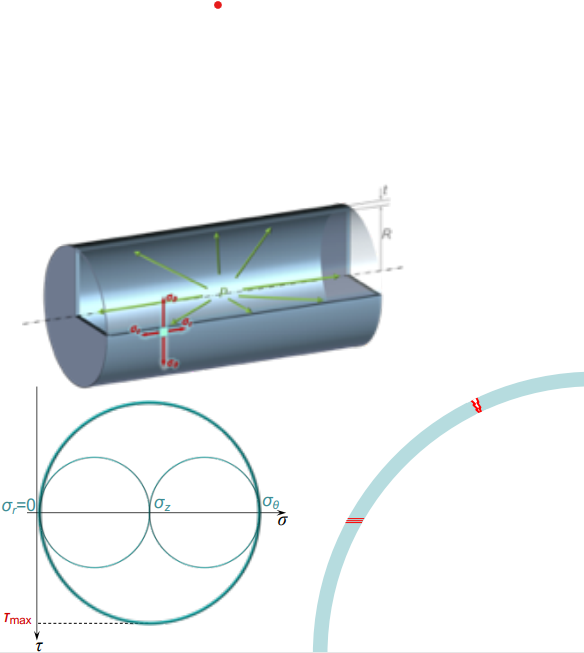
\includegraphics[width = 0.5 \textwidth]{../img/diagram105.png}
  \caption{}
\end{figure}
\subsubsection{Psychrometric Chart:}
\begin{itemize}[noitemsep]
  \item Graphical relationship between: $T_{db}$, $T_{wb}$, $T_{dp}$, $\omega$, $\phi$, $h$, $v$
  \item Constructed for pressure at 1 bar
  \item Valid for mixture pressure around 1 bar, for engineering analysis
  \item Useful for visualizing air-water vapour processes at constant pressure
  \item The specific volume $(v=V/m_a)$ has the unit of $\si{\metre\cubed\per\kilogram}$ dry air
  \item $h$ gives the mixture enthalpy per unit mass of dry air in the mixture:
  \begin{gather}
    h = \frac{H}{m_a} = h_a + \omega h_v \ (\si{\kilo\joule\per\kilogram} \ \text{dry air})
  \end{gather}
\end{itemize}
\begin{figure}[H]
  \centering
  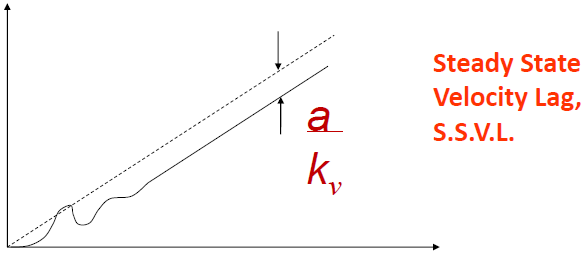
\includegraphics[width = 0.85 \textwidth]{../img/diagram106.png}
  \caption{}
\end{figure}
\section{Psychrometric Applications}
\subsection{Summer and Winter Comfort Zones}
\textbf{Comfort zones:} Acceptable ranges of operative temperature and humidity for people in typical summer and winter clothing during primarily sedentary activity. \\\\
\textbf{Air-conditioning:} To change the temperature and water vapour fraction in the moist air
\begin{figure}[H]
  \centering
  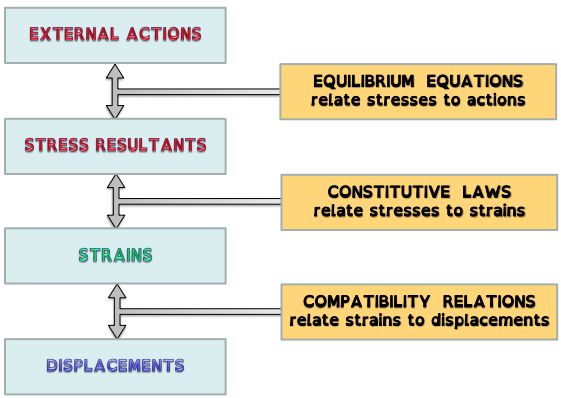
\includegraphics[width = 0.55 \textwidth]{../img/diagram107.png}
  \caption{}
\end{figure}
\subsection{List of Psychrometric Applications}
\begin{itemize}[noitemsep]
  \item Cooling with and without Dehumidification
  \item Cooling with Dehumidification and Reheating
  \item Evaporative Cooling
  \item Humidification
  \item Humidification with Heating
  \item Adiabatic Mixing
  \item Cooling Tower
\end{itemize}
The first 5 of these applications are known of \textbf{Refrigerant, Air-Conditioning Processes}.
\subsection{Air-Conditioning Processes}
\begin{itemize}[noitemsep]
  \item Simple Heating and Cooling ($\omega$=constant), no change in the amount of water vapour.
  \item Cooling with Dehumidification
  \item Heating with Humidification
\end{itemize}
\begin{figure}[H]
  \centering
  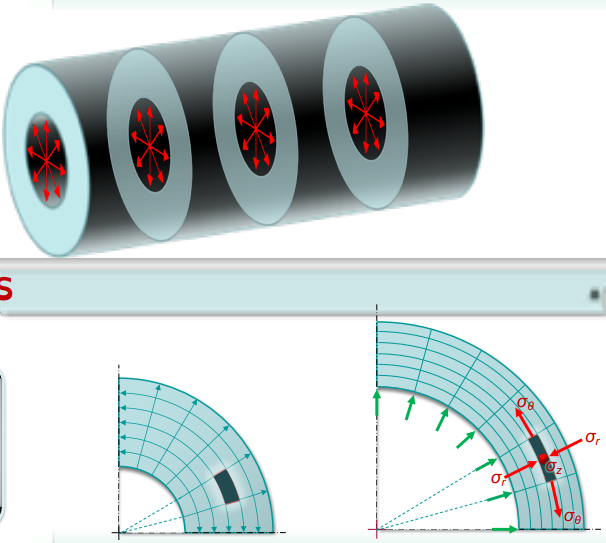
\includegraphics[width = 0.55 \textwidth]{../img/diagram108.png}
  \caption{}
\end{figure}
\subsubsection{Mass and Energy Balance for Open Systems:}
Mass balance for multiple inlets and exits:
\begin{gather}
  \frac{\dif m_{cv}}{\dif t} = \sum_{i}\dot{m}_i - \sum_{e}\dot{m}_e
\end{gather}
Energy balance for multiple inlets and exits:
\begin{gather}
  \frac{\dif E_{cv}}{\dif t} = \dot{Q}_{cv} + \dot{W}_{cv} + \sum_{i}\dot{m}_i\left(h_i + \frac{V_i^2}{2} + gz_i\right) - \sum_{e}\dot{m}_e\left(h_e + \frac{V_e^2}{2} + gz_e\right)
\end{gather}
Steady state:
\begin{gather}
  \frac{\dif m_{cv}}{\dif t} = 0 \\[5pt]
  \frac{\dif E_{cv}}{\dif t} = 0
\end{gather}
\begin{figure}[H]
  \centering
  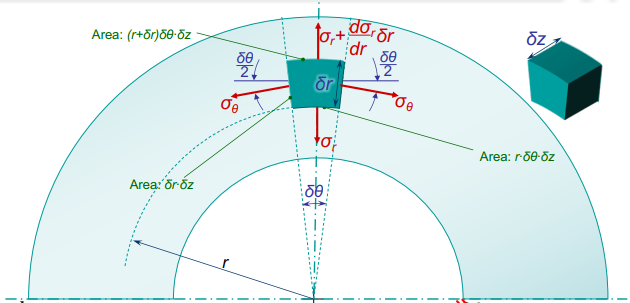
\includegraphics[width = 0.5 \textwidth]{../img/diagram109.png}
  \caption{}
\end{figure}
\subsubsection{Air-Conditioning Processes:}
\begin{figure}[H]
  \centering
  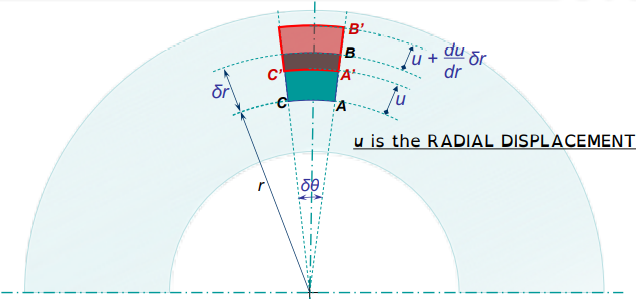
\includegraphics[width = 0.65 \textwidth]{../img/diagram110.png}
  \caption{}
\end{figure}
\begin{itemize}[noitemsep]
  \item On control volume basis;
  \item Steady State;
  \item Assume 
  \begin{itemize}[noitemsep]
    \item $W_{cv} = 0$
    \item $\Delta KE = 0$
    \item $\Delta PE = 0$
  \end{itemize}
  \item Heat transfer between the control volume and its surroundings;
  \item Liquid water (mist) or vapour added
\end{itemize}
Mass Balance:
\begin{gather}
  \dot{m}_{a1} = \dot{m}_{a2} = \dot{m}_{a} \ \ \ \ \ \text{(dry air)} \\[5pt]
  \dot{m}_{v1} + \dot{m}_{w} = \dot{m}_{v2} \ \ \ \ \ \text{(water)} \\[5pt]
  \dot{m}_{v1} = \omega_1\dot{m}_{a} \ \ \text{and} \ \ \dot{m}_{v2} = \omega_2\dot{m}_{a} \\[5pt]
  \therefore \dot{m}_{w} = \dot{m}_{a}(\omega_2 - \omega_1) \ \ \ \ \ \text{(water)}
\end{gather}
Energy Balance:
\begin{gather}
  0 = \dot{Q}_{cv} + (\dot{m}_{a}h_{a1} + \dot{m}_{v1}h_{v1}) + \dot{m}_{w}h_{w} - (\dot{m}_{a}h_{a2} + \dot{m}_{v2}h_{v2}) \\[5pt]
  0 = \dot{Q}_{cv} + \dot{m}_{a}\left[(h_{a1} + \omega_1h_{v1}) + (\omega_2-\omega_1)h_{w} - (h_{a2} + \omega_2h_{v2})\right] \\[5pt]
  0 = \dot{Q}_{cv} + \dot{m}_{a}[h_1 + (\omega_2-\omega_1)h_{w} - h_2]
\end{gather}
The $(h_{a1} + \omega_1h_{v1})$ term represents the \textbf{total specific enthalpy of the mixture} at Point 1, and the $(h_{a2} + \omega_2h_{v2})$ term represents the \textbf{total specific enthalpy of the mixture} at Point 2. They can be simplified by writing in $h_1$ and $h_2$ respectively. The quantities $h_1$ and $h_2$ can be obtained from the Psychrometric Chart, while the entropy of water, $h_w$, can be obtained from the Property Tables. \\\\
Alternatively, enthalpies of the water vapour can be treated as the saturated vapour enthalpies at the corresponding temperatures:
\begin{gather}
  h_{v1} \approx h_{g1} \\[5pt]
  0 = \dot{Q}_{cv} + \dot{m}_{a}\left[(h_{a1} - h_{a2}) + \omega_1h_{g1} + (\omega_2-\omega_1)h_{w} - \omega_2h_{g2}\right] 
\end{gather}
All the properties above can be found from the relevant tables:
\begin{itemize}
  \item $(h_{a1} - h_{a2}) \longrightarrow$ Dry Air: Table A-22 | OR: $h_2-h_1 = c_p(T_2-T_1)$
  \item $\omega_1h_{g1} + (\omega_2-\omega_1)h_{w} - \omega_2h_{g2} \longrightarrow$ Steam Table
\end{itemize}
\subsection{Cooling with and without Dehumidification}
Refrigeration:
\begin{itemize}[noitemsep]
  \item During the evaporation of the refrigerant, heat is absorbed from an air stream
  \item Air side process = cooling process with or without dehumidification
  \item Dehumidification occurs only if air stream temperature drops below dew point temperature
  \item Otherwise, air side process = cooling process at constant humidity ratio
\end{itemize}
Analysis:
\begin{itemize}[noitemsep]
  \item \textbf{Dry coil analysis:} no dehumidification, air stream temperature stays above dew point temperature of incoming air stream
  \item \textbf{Wet coil analysis:} dehumidification, air stream temperature drops below dew point temperature of incoming air stream
\end{itemize}

\subsection*{Cooling without Dehumidification}
\subsubsection{Cooling Process, Dry Coil Analysis:}
Assumptions:
\begin{itemize}[noitemsep]
  \item $\Delta KE = \Delta PE = 0$
  \item Steady state
\end{itemize}
\begin{figure}[H]
  \centering
  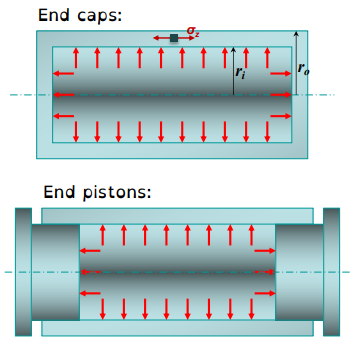
\includegraphics[width = 0.75 \textwidth]{../img/diagram111.png}
  \caption{}
\end{figure}
\begin{align}
  \text{Dry air mass balance:} \ \ \ \ \ &\dot{m}_{a,1} = \dot{m}_{a,2} = \dot{m}_{a} \\[5pt]
  \text{Water mass balance:} \ \ \ \ \ &\dot{m}_{a}\omega_1 = \dot{m}_{a}\omega_2 \\[5pt]
  \text{Energy balance:} \ \ \ \ \ &\dot{Q} = \dot{m}_{a}(h_2-h_1)
\end{align}
\begin{figure}[H]
  \centering
  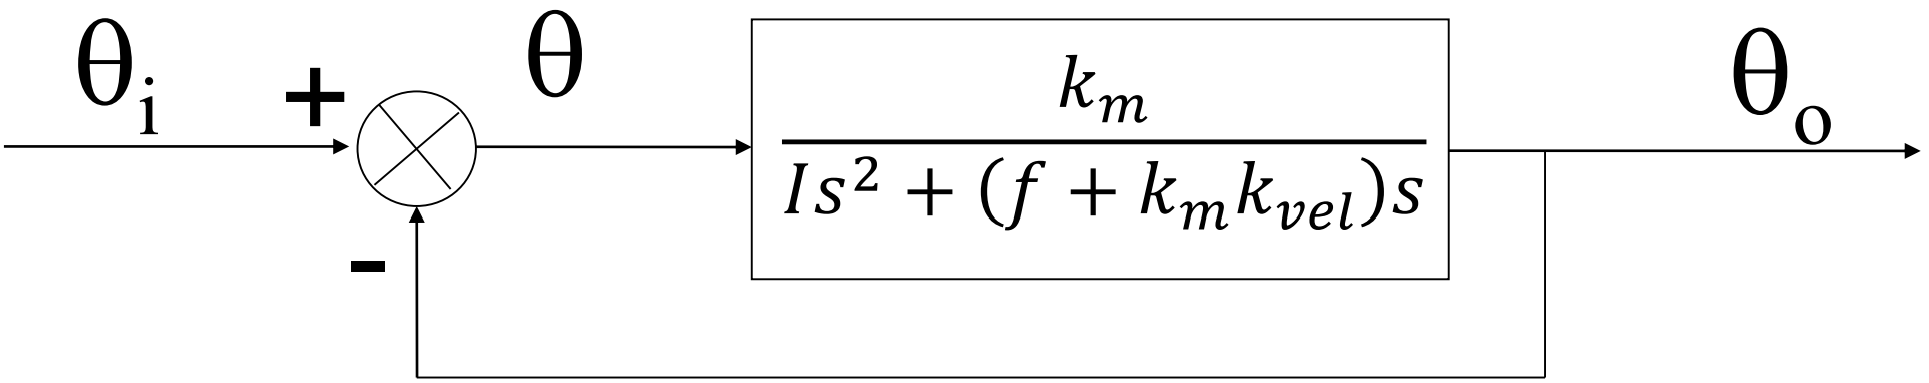
\includegraphics[width = 0.72 \textwidth]{../img/diagram112.png}
  \caption{}
\end{figure}
\subsection*{Cooling with Dehumidification}
\subsubsection{Cooling Process, Wet Coil Analysis:}
Assumptions:
\begin{itemize}[noitemsep]
  \item $\Delta KE = \Delta PE = 0$
  \item Steady state
\end{itemize}
\begin{figure}[H]
  \centering
  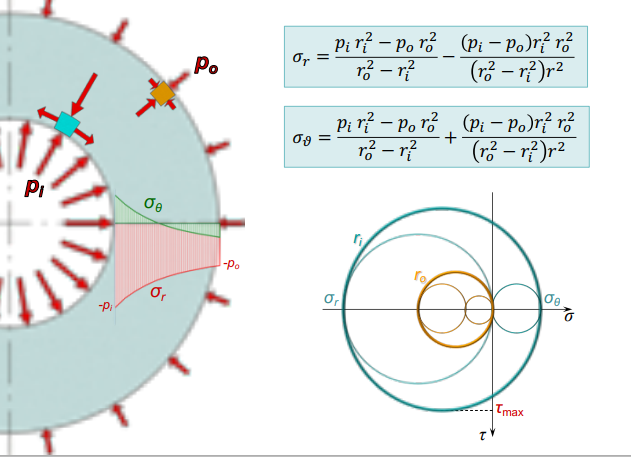
\includegraphics[width = 0.5 \textwidth]{../img/diagram113.png}
  \caption{}
\end{figure}
\begin{align}
  \text{Dry air mass balance:} \ \ \ \ \ &\dot{m}_{a,1} = \dot{m}_{a,2} = \dot{m}_{a} \\[5pt]
  \text{Water mass balance:} \ \ \ \ \ &\dot{m}_{a}\omega_1 = \dot{m}_{a}\omega_2 + \dot{m}_{w} \\[5pt]
  \longrightarrow \ \ &\dot{m}_{w} = \dot{m}_{a}(\omega_1-\omega_2)\\[5pt]
  \text{Energy balance:} \ \ \ \ \ &\dot{Q} = \dot{m}_{a}(h_2-h_1) + \dot{m}_{w}h_{w} \\[5pt]
  &= \dot{m}_{a}\left[(h_2-h_1) + (\omega_1-\omega_2)h_{w}\right]
\end{align}
Note - Outlet state is saturated: $\phi_2 = 1.0$
\begin{figure}[H]
  \centering
  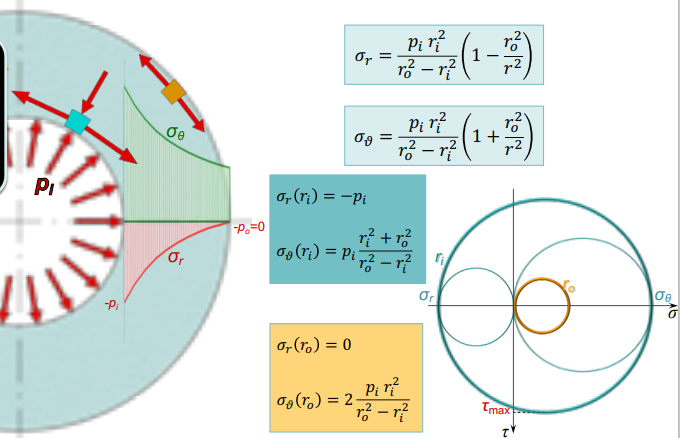
\includegraphics[width = 0.7 \textwidth]{../img/diagram114.png}
  \caption{}
\end{figure}
\textbf{Real} air coil with dehumidification:
\begin{itemize}[noitemsep]
  \item Bulk air stream temperature between two fins may not reach dew point temperature $\longrightarrow$ no dehumidification
  \item Air stream temperature close to the fin surface drops below dew point temperature $\longrightarrow$ dehumidification
  \item Combined air stream leaving the coil may not be saturated!
\end{itemize}
\begin{figure}[H]
  \centering
  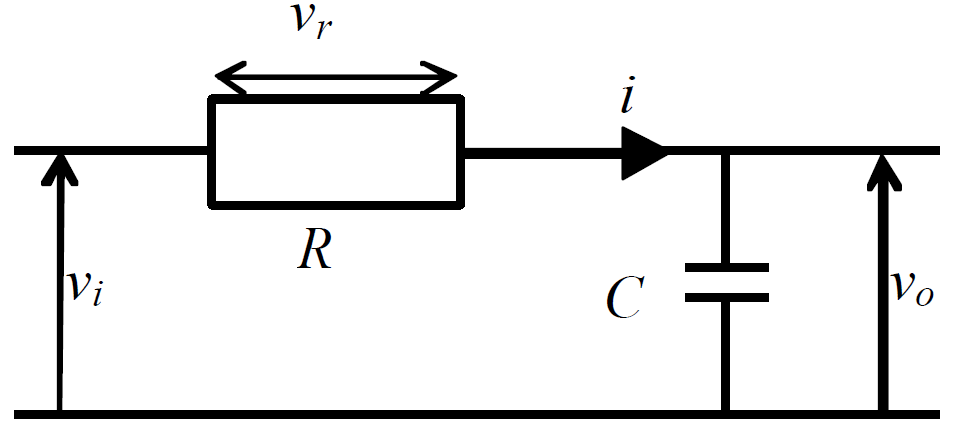
\includegraphics[width = 0.7 \textwidth]{../img/diagram115.png}
  \caption{}
\end{figure}
\begin{figure}[H]
  \centering
  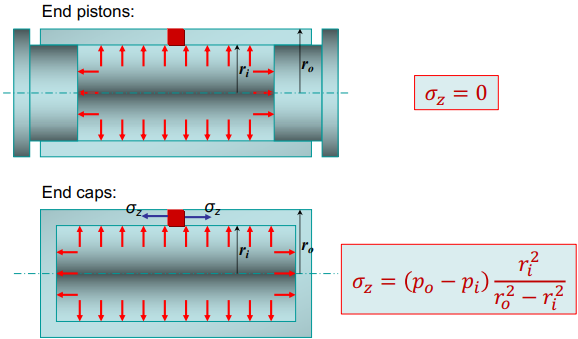
\includegraphics[width = 0.7 \textwidth]{../img/diagram116.png}
  \caption{}
\end{figure}
\subsection{Humidification}
Difference with respect to evaporative cooling (Use water vapour (steam) instead of liquid water to humidify the air) \\\\
Assumptions: 
\begin{itemize}[noitemsep]
  \item $\Delta KE = \Delta PE = 0$
  \item Steady state
  \item $p =$ constant
\end{itemize}
\begin{figure}[H]
  \centering
  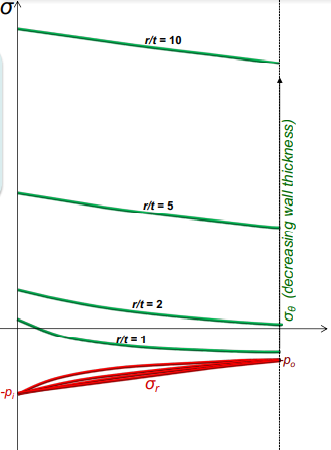
\includegraphics[width = 0.65 \textwidth]{../img/diagram117.png}
  \caption{}
\end{figure}
Mass Balances:
\begin{gather}
  \dot{m}_{a,2} = \dot{m}_{a,3} = \dot{m}_{a} \ \ \ \ \ \text{(dry air)} \\[5pt]
  \dot{m}_{w} = \dot{m}_{a}(\omega_3-\omega_2) \ \ \ \ \ \text{(water)}
\end{gather}
Energy Balance:
\begin{gather}
  h_3 = h_2 + (\omega_3-\omega_2)h_{st}
\end{gather}
For Steam Humidification:
\begin{gather}
  h_{st} = h_{vapour}(T_{st};p_{st}) \longrightarrow T_3>T_2
\end{gather}
For Evaporative Cooler:
\begin{gather}
  h_{st} = h_{w} = h_{f}(T_3) \longrightarrow T_3<T_2
\end{gather}
\begin{figure}[H]
  \centering
  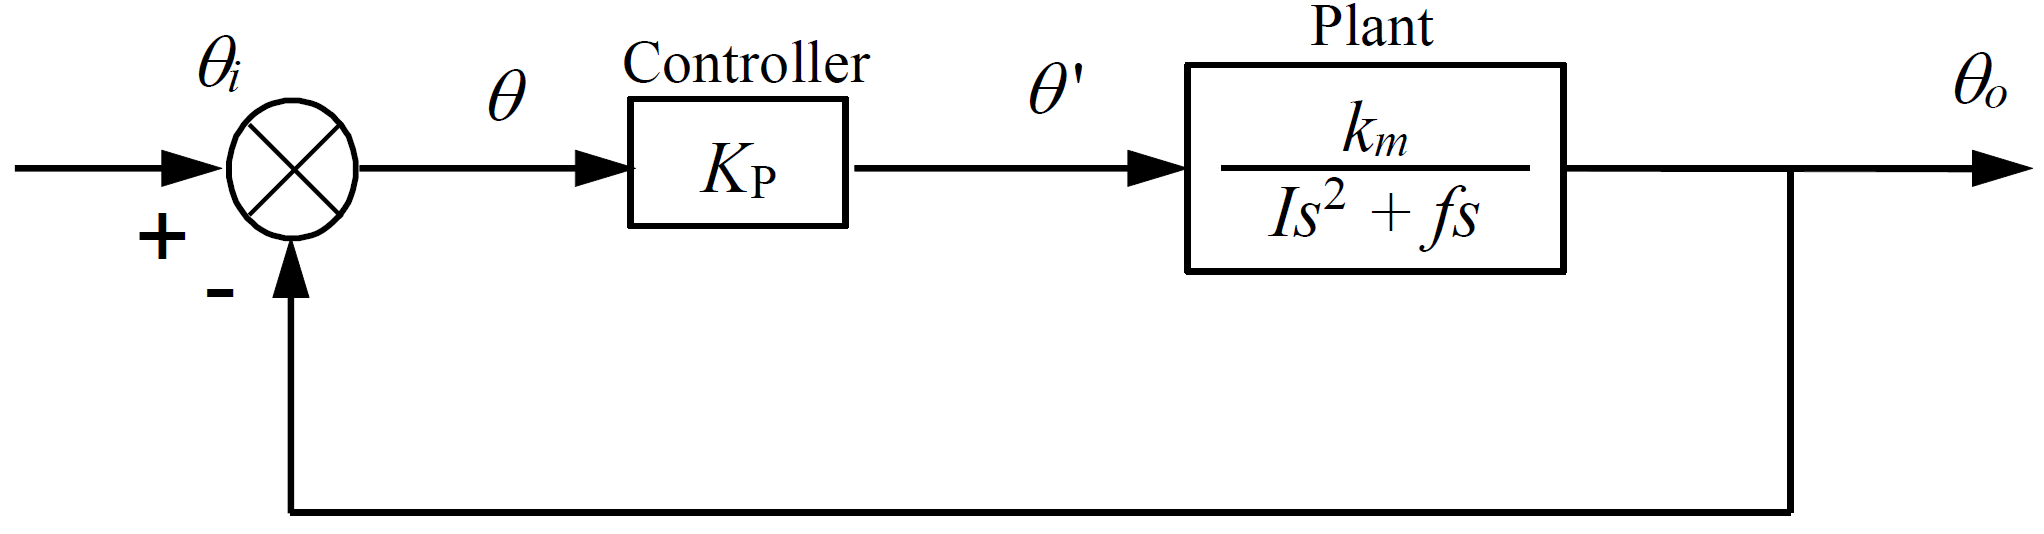
\includegraphics[width = 0.6 \textwidth]{../img/diagram118.png}
  \caption{}
\end{figure}
\subsection{Humidification with Heating}
During winter time, when the outdoor humidity is low, typically \textbf{both} heating and humidification are needed in door.
\begin{figure}[H]
  \centering
  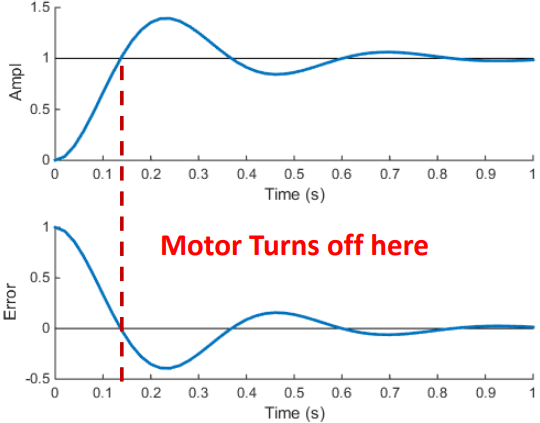
\includegraphics[width = 0.85 \textwidth]{../img/diagram119.png}
  \caption{}
\end{figure}
Heating Coil:
\begin{itemize}[noitemsep]
  \item Hot water
  \item Steam
  \item Combustion gases
  \item Electric heater
\end{itemize}
Dry air mass balance:
\begin{gather}
  \dot{m}_{a,1} = \dot{m}_{a,2} = \dot{m}_{a,3} = \dot{m}
\end{gather}
Water mass balance:
\begin{gather}
  \omega_1\dot{m}_{a} = \omega_2\dot{m}_{a} \longrightarrow \omega_1 = \omega_2 \\[5pt]
  \omega_2\dot{m}_{a} + \dot{m}_{st} = \omega_3\dot{m}_{a} \longrightarrow \dot{m}_{st} = \dot{m}_{a}(\omega_3-\omega_2)
\end{gather}
Energy balance on heater:
\begin{gather}
  \dot{Q}_{heat} = \dot{m}_{a}(h_2-h_1)
\end{gather}
Energy balance on humidification:
\begin{gather}
  h_3 = h_2 + (\omega_3-\omega_2)h_{st}
\end{gather}
\begin{figure}[H]
  \centering
  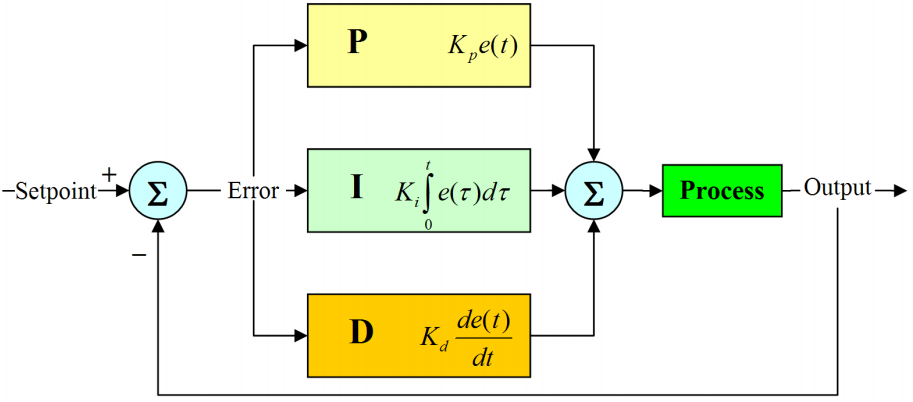
\includegraphics[width = 0.6 \textwidth]{../img/diagram120.png}
  \caption{}
\end{figure}
\subsection{Evaporative Cooling}
Used in desert climates, where it is hot and dry (low relative humidity). \\\\
Analysis is just like \textbf{adiabatic saturator} analysis, except that the supply water temperature is independent of saturation temperature. \\\\
Assumptions:
\begin{itemize}[noitemsep]
  \item $\Delta KE = \Delta PE = 0$
  \item Steady state
  \item $p =$ constant
\end{itemize}
\begin{figure}[H]
  \centering
  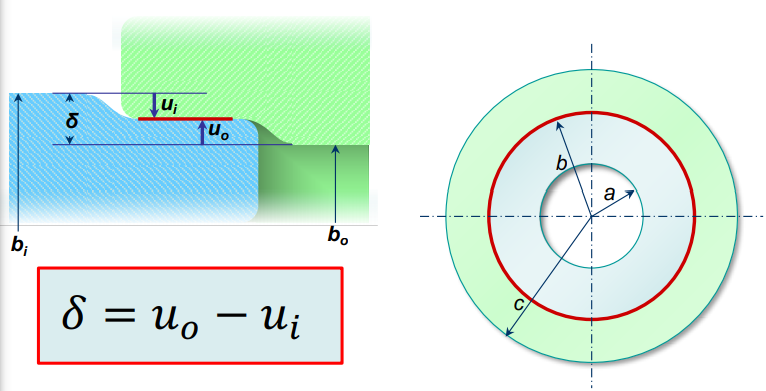
\includegraphics[width = 0.75 \textwidth]{../img/diagram121.png}
  \caption{}
\end{figure}
Mass Balances:
\begin{gather}
  \dot{m}_{a,1} = \dot{m}_{a,2} = \dot{m}_{a} \ \ \ \ \ \text{(dry air)} \\[5pt]
  \dot{m}_{w} = \dot{m}_{a}(\omega_2-\omega_1) \ \ \ \ \ \text{(water)}
\end{gather}
Energy Balance:
\begin{gather}
  (h_{a2} + \omega_2h_{v2}) = (h_{a1} + \omega_1h_{v1}) + (\omega_2-\omega_1)h_{f} \\[5pt]
  h_2 = h_1 + (\omega_2-\omega_1)h_f
\end{gather}
The $(\omega_2-\omega_1)h_f$ term is much smaller than the other two terms:
\begin{gather}
  \therefore h_2 \approx h_1 \ \ \ \text{is a good approximation} \\[5pt]
  \therefore h \approx \text{constant} \ \ \ \& \ \ \ T_{wb} \approx \text{constant}
\end{gather}
\begin{figure}[H]
  \centering
  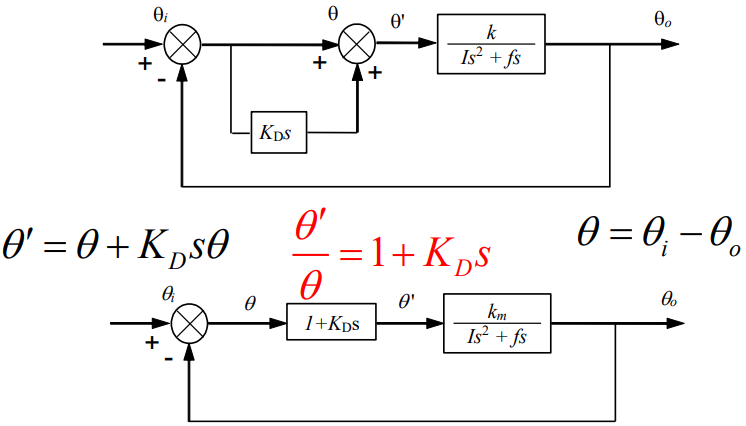
\includegraphics[width = 0.7 \textwidth]{../img/diagram122.png}
  \caption{}
\end{figure}
\subsection{Adiabatic Mixing of Two Moist Air Streams}
\textbf{Adiabatic Mixing} of state 1 and state 2:
\begin{itemize}[noitemsep]
  \item Assume:
  \begin{itemize}[noitemsep]
    \item $\dot{Q} = 0$
    \item $\dot{W} = 0$
  \end{itemize}
  \item Mixing state is \textbf{on a straight line} between the two inlet state points
\end{itemize}
\begin{figure}[H]
  \centering
  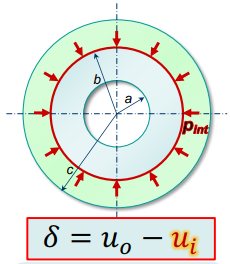
\includegraphics[width = 0.5 \textwidth]{../img/diagram123.png}
  \caption{}
\end{figure}
Dry air mass balance:
\begin{gather}
  \dot{m}_{a,3} = \dot{m}_{a,1} + \dot{m}_{a,2}
\end{gather}
Vapour mass balance:
\begin{gather}
  \omega_3\dot{m}_{a,3} = \omega_1\dot{m}_{a,1} + \omega_2\dot{m}_{a,2}
\end{gather}
Energy balance:
\begin{gather}
  h_3\dot{m}_{a,3} = h_1\dot{m}_{a,1} + h_2\dot{m}_{a,2} \\[5pt]
  \frac{\dot{m}_{a1}}{\dot{m}_{a2}} = \frac{\omega_2-\omega_3}{\omega_3-\omega_1} = \frac{h_2-h_3}{h_3-h_1}
\end{gather}
\begin{figure}[H]
  \centering
  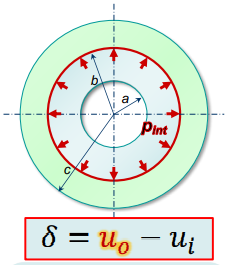
\includegraphics[width = 0.6 \textwidth]{../img/diagram124.png}
  \caption{}
\end{figure}
\subsection{Cooling Towers}
\begin{itemize}[noitemsep]
  \item Cooling towers are used to:
  \begin{enumerate}[noitemsep]
    \item Release power plant waste heat at acceptable $T$ to surroundings
    \item Provide chilled water
  \end{enumerate}
  \item Operate by natural or forced convection of air
  \item Counterflow, cross flow or hybrid configuration
\end{itemize}
\begin{figure}[H]
  \centering
  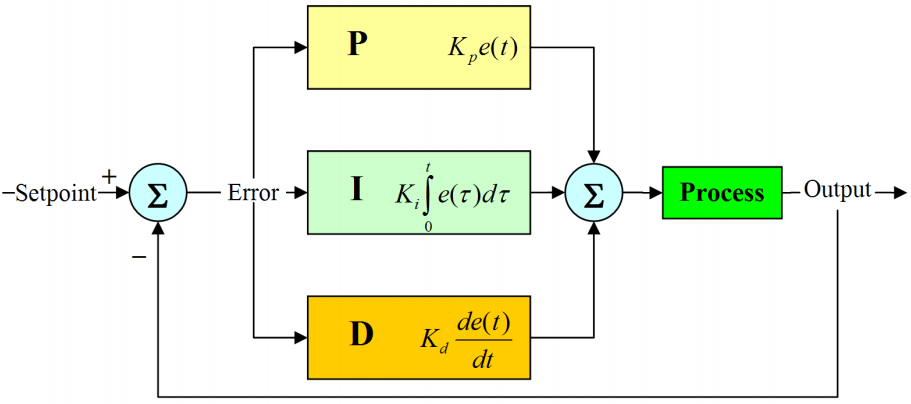
\includegraphics[width = 0.9 \textwidth]{../img/diagram125.png}
  \caption{Left: An induced-draft counterflow cooling tower \ \ | \ \ Right: A natural-draft cooling tower}
\end{figure}
\begin{itemize}[noitemsep]
  \item Steady state analysis of mass and energy balance, usually;
  \item Heat transfer to surroundings is neglected, usually.
  \item Fan power may be considered
\end{itemize}
\begin{figure}[H]
  \centering
  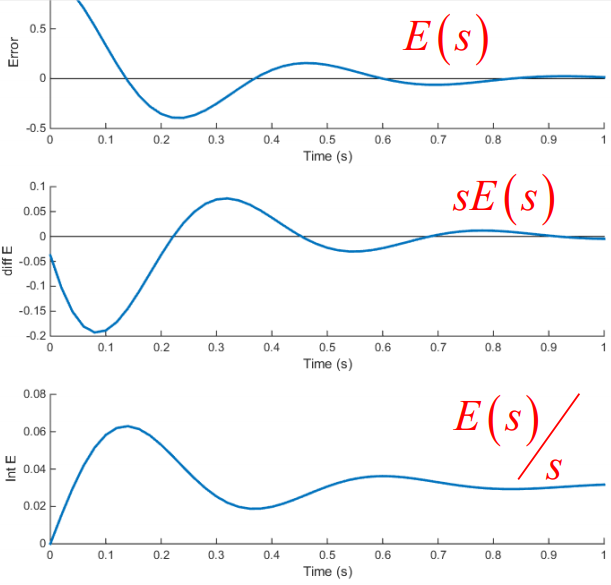
\includegraphics[width = 0.53 \textwidth]{../img/diagram126.png}
  \caption{}
\end{figure}
\end{document}